\documentclass[mathserif,9pt]{beamer}
\hypersetup{pdfmode=FullScreen}
\usepackage{pst-plot, pstricks,pstricks-add,pst-node, pst-tree}
\usepackage[]{german}
%\usepackage{pgfpages}
%\usepackage{qtree}

\mode<presentation>
{
  \usetheme{shadow}
  \usecolortheme{crane}
  \setbeamercovered{transparent}
  \useoutertheme{infolines}
}

\usepackage{times}
\usepackage{graphicx}
\usepackage[T1]{fontenc}
\usepackage{amssymb,amsmath,amsthm, amsbsy, bm}
\usepackage{enumerate}
\newcommand{\bs}{\boldsymbol}
\newcommand{\dd}{\mathrm{d}}
\beamertemplatenavigationsymbolsempty
\DeclareMathOperator{\maximize}{maximize}
\DeclareMathOperator{\E}{\mathbb{E}}
\DeclareMathOperator{\V}{V\mathbb{V}}
\DeclareMathOperator{\VaR}{VaR}
\DeclareMathOperator{\CVaR}{CVaR}

\title[Werden die grossen Spieler genug Kapazit�ten bauen?] 
{Generation Capacity Investment in Electricity Markets in an Oligopolistic, Dynamic and Stochastic Framework}

\author[Anton Burger\and Robert Ferstl]{Anton Burger\inst{1} \and Robert Ferstl\inst{2}}


\institute[]{
\inst{1}Institute for Regulatory Economics\\
Vienna University of Economics and Business Administration
\and
\inst{2}Department of Finance\\
University of Regensburg}

\date[EnInnov08]{\scriptsize\em \textbf{10. Symposium Energieinnovation - Energiewende\\Graz\\\vspace{0.2cm} 13.-15. Februar 2008}}

\pgfdeclareimage[height=1.0cm]{wu-logo}{wu-logo}
\logo{\pgfuseimage{wu-logo}}	% show logo
%\setbeameroption{show notes}
\setbeameroption{hide notes}

\begin{document}

\frame{\titlepage}

\section<presentation>*{�bersicht}

\begin{frame}
  \frametitle{�bersicht}
  \tableofcontents[pausesections]
\end{frame}


%\AtBeginSubsection[]
%{
%  \begin{frame}<beamer>
%    \frametitle{Outline}
%    \tableofcontents[current,currentsubsection]
%  \end{frame}
%}

\section{Einleitung}

%	\subsection{}
\section{Strommarkt in Deutschland - Daten}
%		\subsection{}
		\begin{frame}{Fakten}
\begin{itemize}
	\item liberalisierte Stromm�rkte
	\item keine zentrale Planung mehr sondern dezentrale Marktentscheidungen
\end{itemize}

Besonderheiten in Bezug auf Investitionen:

\begin{itemize}  
	\item sehr grosse Spieler $\rightarrow$ Oligopolsituation
\begin{itemize}
	\item Herfindahl Hirschman Index $> 2000$ (Brunekreeft (2006))
	\item RWE, E.ON, Vattenfall und EnBW  
\end{itemize}
	\item hohe Preisvolatilit�t $\rightarrow$ Unsicherheit

	\item L - f�rmiger Kostenverlauf
	\item hohe Investitionskosten mit langer Bauzeit - 2 Stufiges Insvestitionsspiel
\end{itemize}
		\end{frame}		
				
		
	  \begin{frame}{Fakten II}

\begin{figure}[htb]
  \centering
  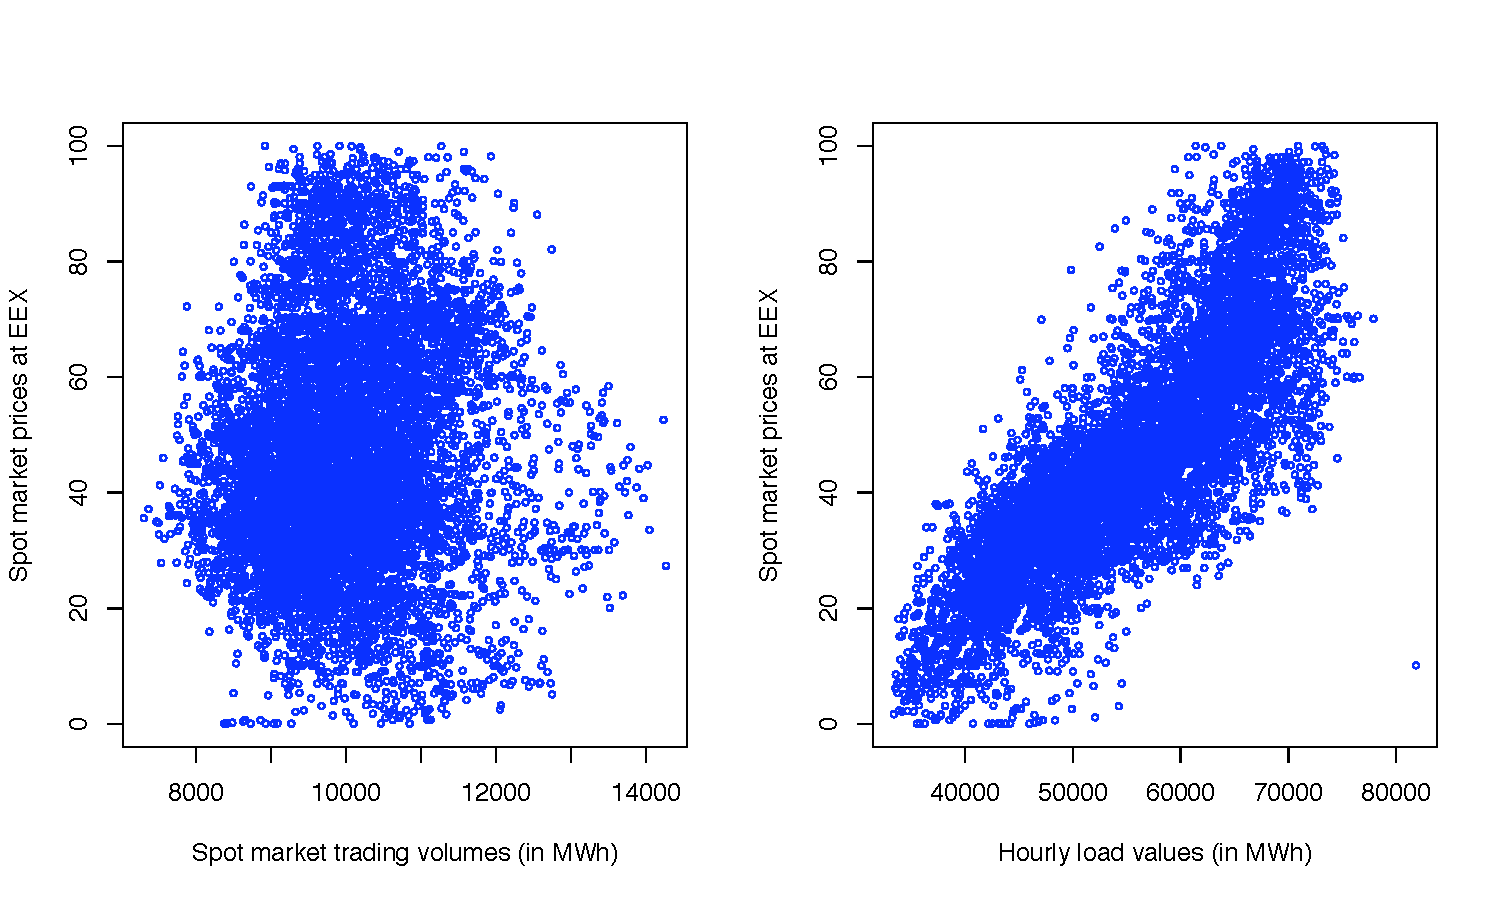
\includegraphics[width=2 in]{pricequant.pdf}
  \label{fig:pricequant}
\\
 \scriptsize Source: EEX, UCTE
\end{figure}
\begin{table}[htb]
\centering
\small
\begin{tabular}{lrrr}
\hline
 & \multicolumn{1}{c}{Occupancy} & \multicolumn{1}{c}{Average price} & \multicolumn{1}{c}{Average quantity}   \\ 
 & \multicolumn{1}{c}{per year} & \multicolumn{1}{c}{(EUR)} & \multicolumn{1}{c}{(MWh)}   \\ 
 \hline
$>$ 100 & \multicolumn{1}{c}{46} & \multicolumn{1}{c}{128} & \multicolumn{1}{c}{83,558}   \\ 
between 80 and 100 & \multicolumn{1}{c}{134} & \multicolumn{1}{c}{86} & \multicolumn{1}{c}{81,493}   \\ 
between 60 and 80 & \multicolumn{1}{c}{788} & \multicolumn{1}{c}{68} & \multicolumn{1}{c}{78,256}   \\ 
between 40 and 60 & \multicolumn{1}{c}{2,174} & \multicolumn{1}{c}{49} & \multicolumn{1}{c}{71,956}  \\ 
between 20 and 40 & \multicolumn{1}{c}{4,201} & \multicolumn{1}{c}{30} & \multicolumn{1}{c}{58,578}  \\ 
below 20 & \multicolumn{1}{c}{1,417} & \multicolumn{1}{c}{14} & \multicolumn{1}{c}{42,627} \\
\hline
 & \multicolumn{1}{c}{8760} &  &    \\ 
 \hline
\end{tabular}
\label{tab:demand}

\scriptsize Source: EEX, UCTE
\end{table}	
\normalsize
		\end{frame}
		
\section{Motication und Literatur}		
		\begin{frame}{Motivation und Literatur}
		
		 \begin{itemize}
		 \item Kann man auf den momentanen Elektizit�tsm�rkten effiziente Investitionen erwarten?
		 
		 \begin{itemize}
		 \item Was bedeutet ausreichend? $\rightarrow$ Peak Load Pricing (Crew and Kleindorfer (1986))
		 \item Wie wirkt ein Oligopol auf Investitionsentscheidungen? (von der Fehr and Harbord (1995))
		 \item Wird m�glicherweise auch die Technologiewahl verzerrt?
		 \end{itemize}

		 \item Abbildung der tats�chlichen Investitionsentscheidung in einem mehrstufigen Spiel
		 
\begin{itemize}
\item Annahmen �ber Informationen die die Spieler ber�cksichtigen (Cellini und Lambertini (2004))
	\begin{itemize}
	\item Open loop $\rightarrow$ Anfangszustand des Spiels und Zeit
	\item S-adapted Open loop $\rightarrow$ zus�tzlich Realisation der Zufallsvariablen
	\item Closed loop $\rightarrow$ zus�tzlich Ver�nderungen der Statusvariablen
	\end{itemize}
\item Game with Probabilistic Scenarios (GPS) following (Genc (2007))
\end{itemize}
\item Wie weit weicht die tats�chliche von der optimalen Investitionsentscheidung ab?

		\end{itemize}
		\end{frame}


\section{�konomie auf Stromm�rkten}

\begin{frame}
					
\frametitle{optimales Peak Load Pricing unter perfekter Konkurrenz}
\begin{columns}
\begin{column} {0.5\textwidth}
\begin{figure}[h]
\centering
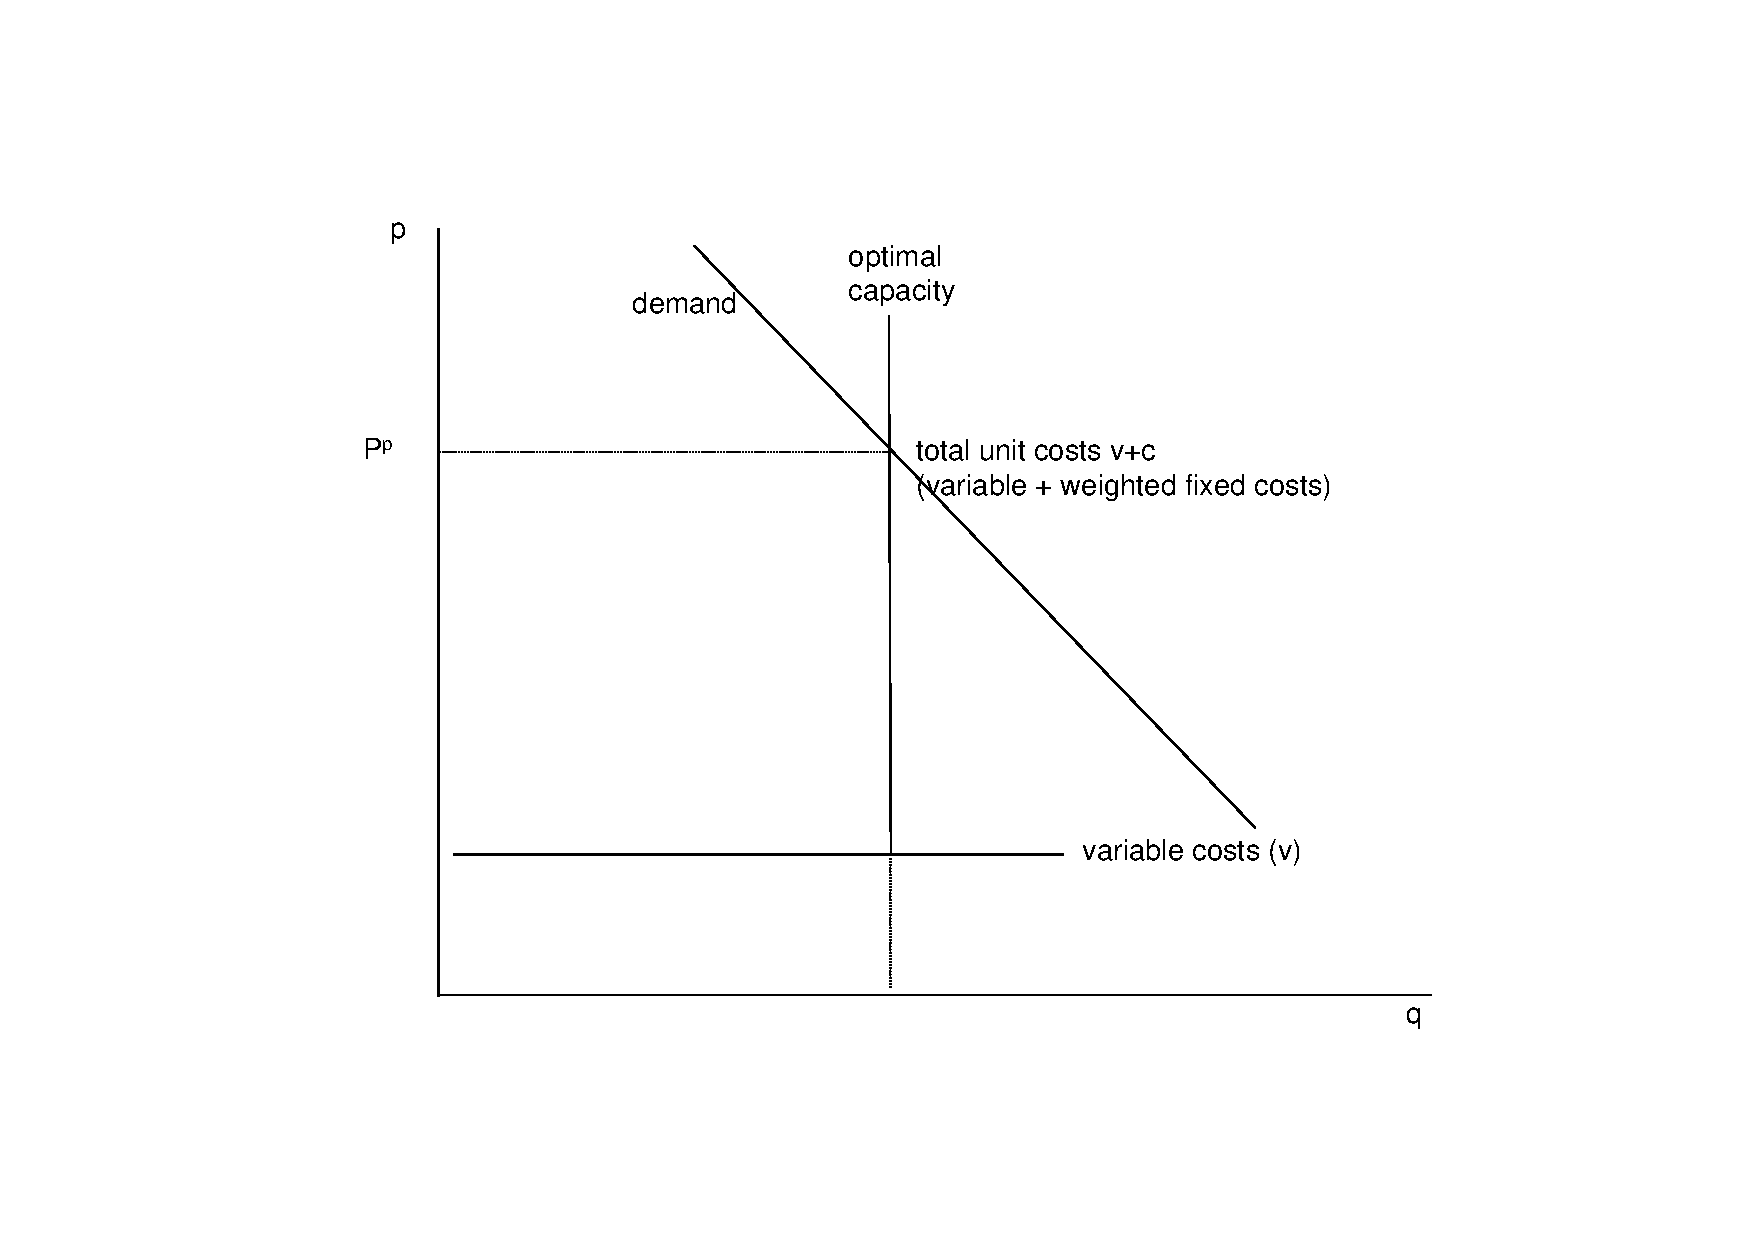
\includegraphics[width=1.\textwidth]{peak_load_opt}
    \caption{von der Fehr and Harbord (1995)}
    \label{fig:Daten 2004}            
\end{figure}
\end{column}

\begin{column} {0.5\textwidth}
\begin{itemize}
\item An der optimalen Kapazit�t ist der marginale Nutzen gleich den marginalen Kosten der Kapazit�t
\end{itemize}

\begin{equation}
	c=(p^p-v)*\pi
\end{equation}

{\small
\begin{tabbing}
whereby: \= $c$ \  \= Kosten einer Einheit Kapazit�t \\
\> $p^p$   \    \> Engpasspreis  \\
\> $v$    \   \> variable Kosten \\
\> $\pi$    \    \> Wahrscheinlichkeit f�r Peak Periode
\end{tabbing}}

\begin{itemize}
\item Genau das w�rde auch eine Firma unter perfekter Konkurrenz tun
\end {itemize}

\end{column}
\end{columns}

\end{frame}
\begin{frame}

\frametitle{Verzerrte Investitionsanreize im Oligopol I}
\begin{columns}
\begin{column} {0.6\textwidth}

\begin{figure}[h]
\centering
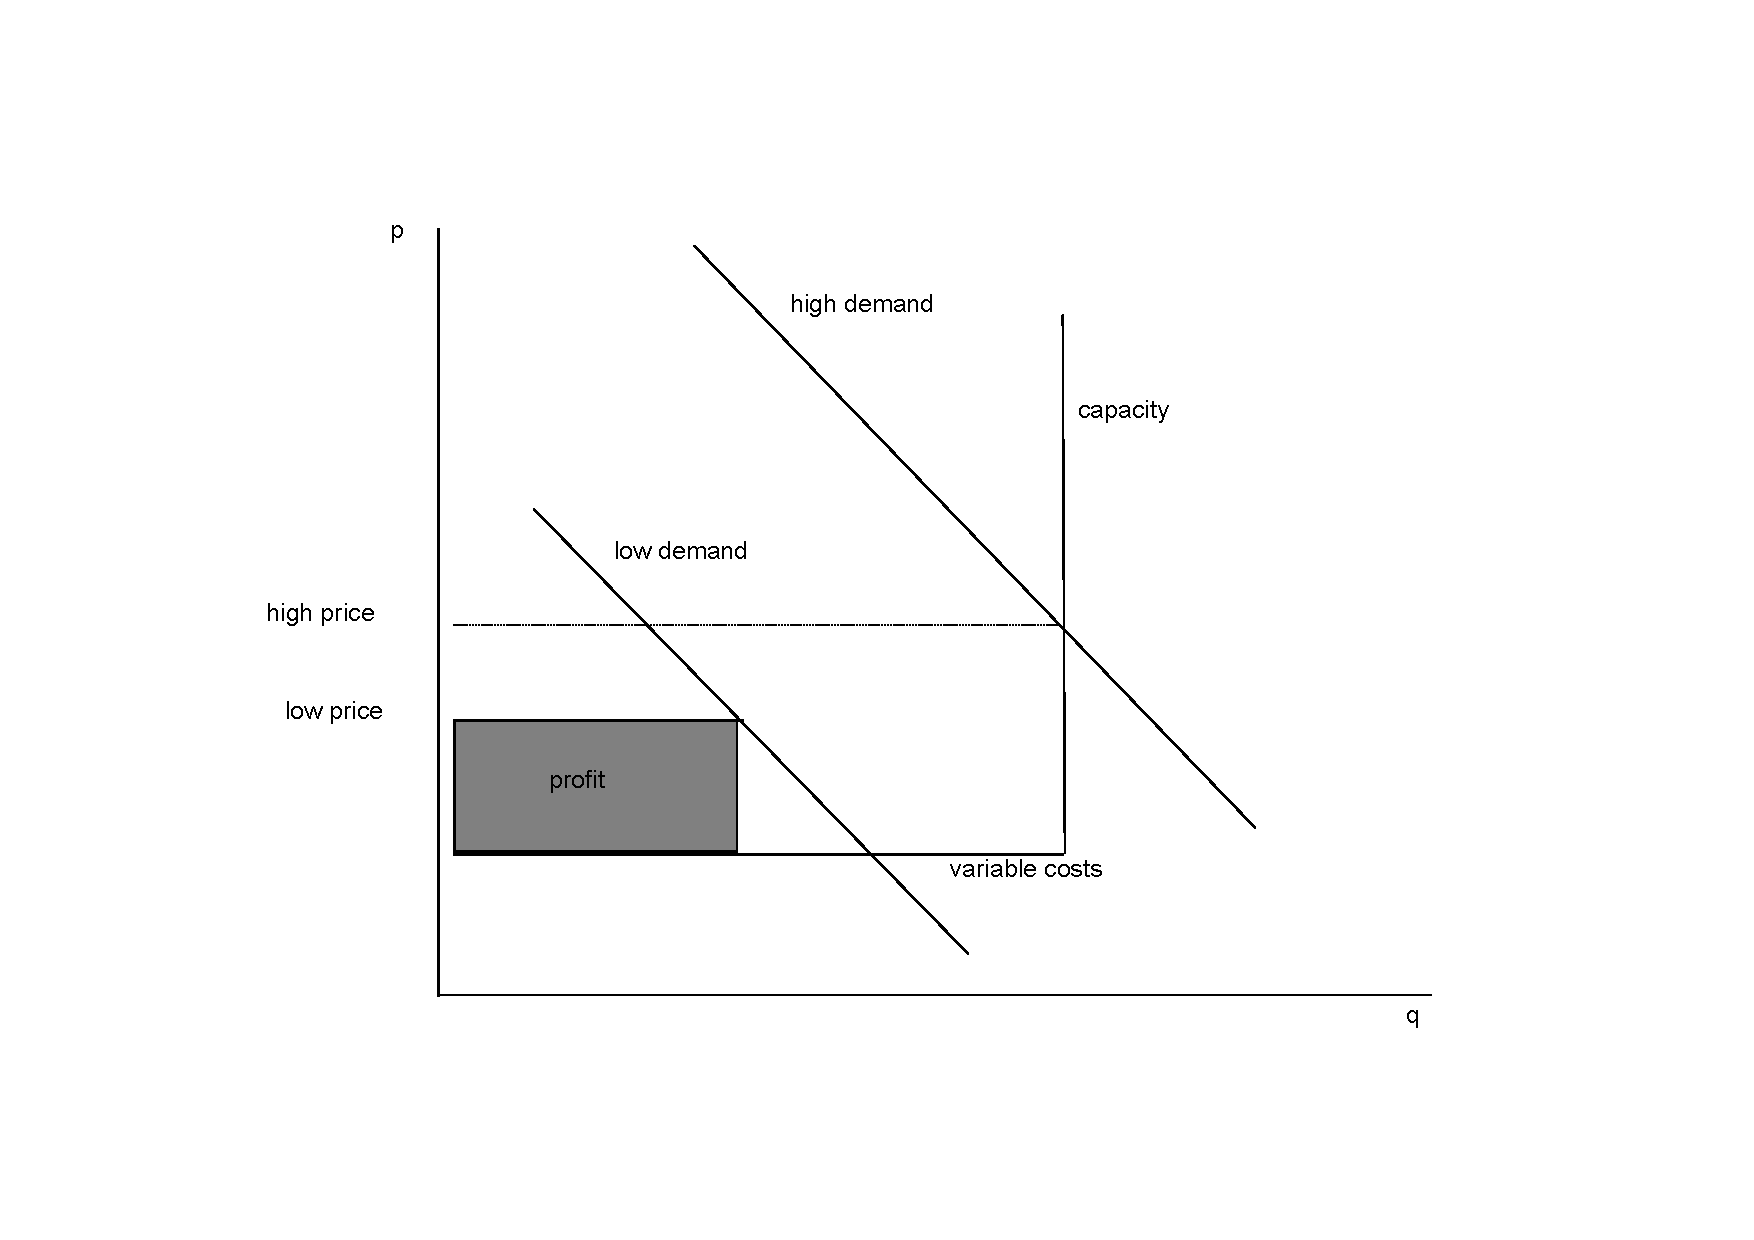
\includegraphics[width=1.\textwidth]{imperfect_spot_pricing}
    \caption{von der Fehr and Harbord (1995)}
    \label{fig:Daten 2004}            
\end{figure}
\end{column}

\begin{column} {0.4\textwidth}
\begin{itemize}
\item preise $>$ als die marginalen kosten
\item zus�tzlicher Investitionsanreiz durch Gewinne in Off-Peak Perioden
\end {itemize}
  
\begin{equation}
	1/2 (1-\pi) (p^{op}-v)
\end{equation} 
{\small
\begin{tabbing}
whereby: \= $p^{op}$ \  \= Off-Peak Preis
\end{tabbing}}

\begin{itemize}
\item optimum gleich wie vorher
\item Verzerrung in Richtung zu viel Investments
\end {itemize}

\end{column}
\end{columns}
	

\end{frame}
\begin{frame}

\frametitle{Verzerrte Investitionsanreize im Oligopol II}
\begin{columns}
\begin{column} {0.6\textwidth}

\begin{figure}[h]
\centering
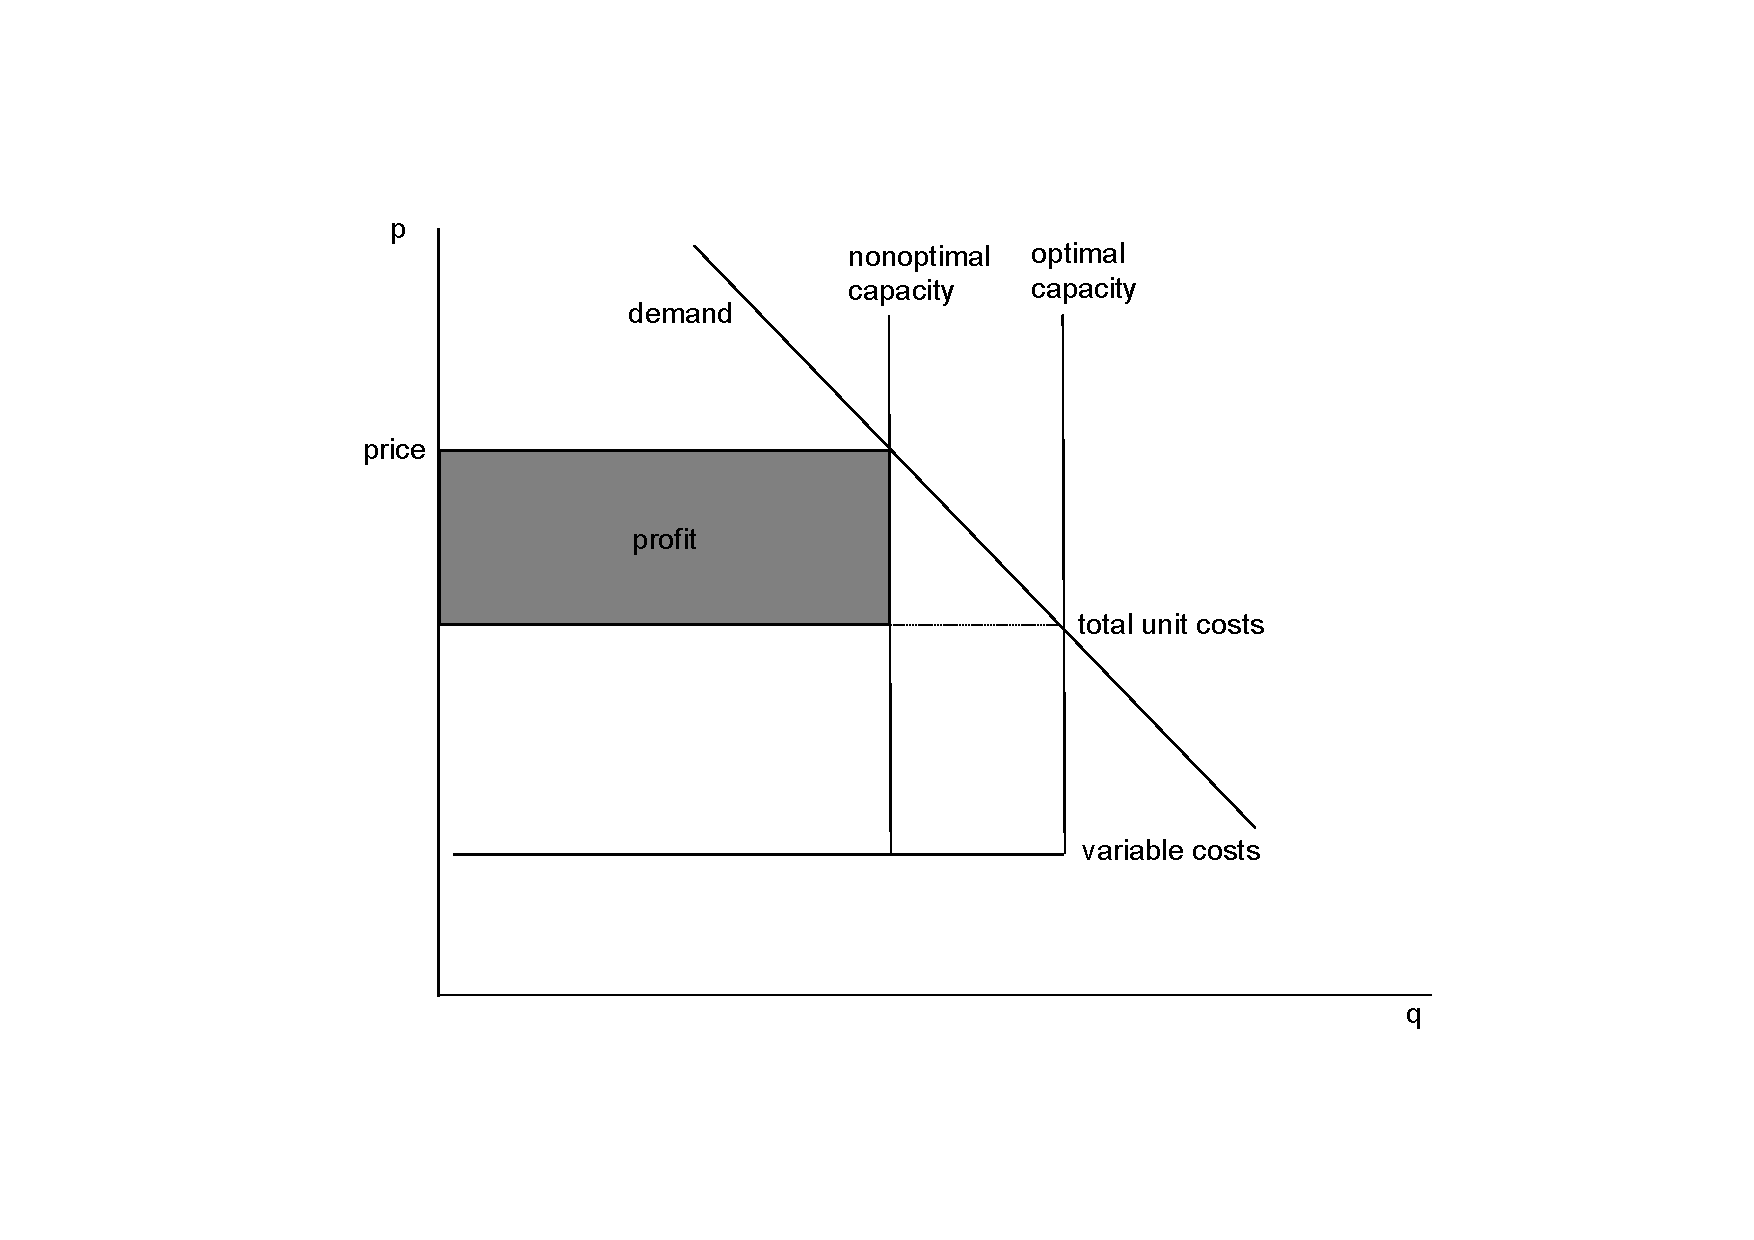
\includegraphics[width=1.\textwidth]{imperfect_spot_pricing2}
    \caption{von der Fehr and Harbord (1994)}
   % \label{fig:Daten 2004}            
\end{figure}
\end{column}

\begin{column} {0.4\textwidth}
\begin{itemize}
\item wenn man weniger investiert, erh�ht sich der Preis in Peak-Periods
\end {itemize}

\begin{equation}
\pi (w^p(K)+\frac{\partial w^p(K)}{\partial q}-v)
\end{equation}

{\small
\begin{tabbing}
\= $w^p$ \  \= Nachfragefunktion in Peak Perioden \\
\> $K$   \    \> Kapazit�t
\end{tabbing}}

\begin{itemize}
\item die Ver�nderung des Preises durch mehr Kapazit�t wird nun im Oligopol ber�cksichtigt
\item dieser Effekt ist negativ f�r das Unternehmen also Verzerrung Richtung zu wenig Investments
\end {itemize}

\end{column}
\end{columns}
\end{frame}

\section{Modell}

		\begin{frame}{Modell}
\begin{gather}
	\max \pi_i(q_{i,k}^{s,m,t},K^t_{i,k},I_{i,k})=
	\sum_{m\in M} v_m \left[ (\alpha_m^l-\beta_m^l \sum_{i\in N}\sum_{k\in K} q_{i,k}^{l,m,1}) \sum_{k\in K} q_{i,k}^{l,m,1} - \sum_{k\in K} c_k q_{i,k}^{l,m,1} \right]  \\  \nonumber 
	+ \delta \sum_{s\in S} p_s \sum_{m\in M} v_m \times  \left[ (\alpha_m^s-\beta_m^s \sum_{i\in N}\sum_{k\in K} q_{i,k}^{s,m,2}) \sum_{k\in K} q_{i,k}^{s,m,2} - \sum_{k\in K} c_k q_{i,k}^{s,m,2}  \right]   \\  \nonumber 
									- \sum_{k\in K} \Gamma_{k\in K} I_{i,k} + \delta \sum_{k\in K} F_k I_{i,k}  \\       
			\text{s.t.:} \  q_{i,k}^{l,m,t} - K^{t}_{i,k} \leq 0; \ \forall i,k,m,t    \label{eq:oligopmax2}\\ 
										  K^{2}_{i,k}  - \rho K^{1}_{i,k}  - I_{i,k} = 0 ; \ \forall i,k  \label{eq:ologopmax5} \\  
\end{gather}
\small
\begin{tabular}[c]{l l l l}
$i\in N$        & players, firms &$K_{i,k}^t$& available capacity\\
$s\in S$       	& scenarios &$q_{i,k}^{s,m,t}$&quantity\\
$m\in M$	& states of the market &$I_{i,k}^t$& investment\\
$k\in K$	& technologies &$p_s$ & probability of scenario $s$\\
$t\in T$	& time &$\delta$& discount factor\\
 
$\rho$   & depreciation factor &$c_k$& variable costs\\
$\alpha_m$  & demand function intercept in market state $m$ &$\Gamma_k$&investment costs \\
$\beta_m$   & demand function slope in market state $m$ &$F_k$&scrap values \\
\end{tabular}
\normalsize
		\end{frame}
\section{Resultate}

\begin{frame}{kurzfristiges Gleichgewicht}
\begin{center}
\small
\begin{tabular}{llrrrrrr}
\hline
\hline
           &            &    exthigh &      vhigh &       high &      inter &        low &       vlow \\
\hline
     t = 0 &            &            &            &            &            &            &            \\
\hline
 olig. &          q &     72,863 &     69,580 &     66,698 &     61,660 &     49,427 &     34,847 \\

           &          p &        210 &        149 &        118 &         83 &         52 &         27 \\
\hline
   opt. &          q &     82,498 &     82,498 &     77,344 &     73,331 &     63,273 &     41,546 \\

           &          p &        136 &         81 &         72 &         44 &         17 &         16 \\
\hline
\hline
     t = 1 &            &            &            &            &            &            &            \\

 olig. &            &            &            &            &            &            &            \\

       low &          q &     75,922 &     72,898 &     70,468 &     65,094 &     52,295 &     35,817 \\

           &          p &        186 &        132 &        102 &         72 &         45 &         26 \\

      high &          q &     79,105 &     76,176 &     72,864 &     67,972 &     54,711 &     37,861 \\

           &          p &        200 &        140 &        112 &         77 &         48 &         26 \\
\hline
   opt. &            &            &            &            &            &            &            \\
       low &          q &     94,509 &     91,497 &     86,167 &     81,578 &     65,952 &     44,771 \\
           &          p &         44 &         34 &         34 &         16 &         11 &         11 \\
           &            &            &            &            &            &            &            \\
      high &          q &     96,839 &     94,397 &     90,860 &     84,879 &     67,284 &     47,327 \\
           &          p &         65 &         44 &         34 &         20 &         16 &         11 \\
\hline
\hline
\end{tabular}  
\normalsize
\end{center}
	\end{frame}


\begin{frame}{Investitionsanreize - Schattenpreise der Kapazit�t}

\small

\begin{tabular}{llrrrrrrr}
\hline
\hline
           &            & extr. high &    v. high &       high &    interm. &        low &     v. low &  {\bf Sum} \\
\hline
       RWE & Hydro Power &        831 &       1970 &       6698 &      18479 &      12603 &       4251 & {\bf 44832} \\

           &    Nuclear &        743 &       1715 &       5201 &      14348 &       4621 &       1559 & {\bf 28188} \\

           &    Lignite &        693 &       1568 &       4334 &      11957 &            &            & {\bf 18552} \\

           &  Hard Coal &        440 &        831 &            &            &            &            & {\bf 1271} \\
\hline
      EnBW & Hydro Power &       5587 &      11512 &      52311 &      90176 &      98341 &      12045 & {\bf 269972} \\

           &    Nuclear &       5500 &      11257 &      50814 &      86045 &      90359 &       9352 & {\bf 253328} \\

           &    Lignite &       5449 &      11110 &      49947 &      83654 &      85738 &       7794 & {\bf 243692} \\

           &  Hard Coal &       5196 &      10373 &      45613 &      71697 &      62633 &            & {\bf 195512} \\

           &        Gas &       4396 &       8041 &      31902 &      33869 &            &            & {\bf 78208} \\

           &        Oil &       3913 &       6634 &      23628 &      11042 &            &            & {\bf 45217} \\

           &   Pump St. &       2257 &       1810 &            &            &            &            & {\bf 4067} \\
\hline
\hline
\end{tabular}
\small
\normalsize
\end{frame}




\begin{frame}{Investitionen - Optimum vs. Oligopol}
\begin{center}
\begin{tabular}{llrrrr}
\hline
\hline
investments &            &            &            & \multicolumn{ 2}{r}{Scen. w. Brown Coal} \\
\hline
 oligopoly &            & Brown Coal &            &    Nuclear &  Hard Coal \\
\hline
           &        EON &       1,063 &            &            &            \\
           &     Vatten &       7,256 &            &       6,249 &        283 \\
           &       EnBW &       9,102 &            &       8,248 &            \\
           &        Sum &      17,422 &            & \multicolumn{ 2}{c}{14,780} \\
\hline
   optimum &            &      31,096 &            &      27,658 &            \\
\hline
\hline
\end{tabular}  
\normalsize
\end{center}
\end{frame}

\section{Conclusio}

%		\subsection{}
		\begin{frame}{Conclusio}

\begin{box}
\begin{itemize}
	\item Untersuchung von Investitionsanreizen auf E-M�rkten ohne Ber�cksichtigung der strategischen Investitionen unm�glich
	\item rein analytisches Modell - zuwenig oder auch zuviel Investitionen
	\item realistisches Beispiel gerechnet
	\item Vergleich zwischen Wohlfahrtsoptimum und Oligopoll�sung zeigt ein Investitionsproblem
	\item durch Kernkraftausstieg und alternde Kapazit�ten noch verschlimmert
\end{itemize}
\end{box}

		\end{frame}	
	

\section{Referenzen}
\scriptsize

\begin{frame}[allowframebreaks]
      \frametitle<presentation>{References}

      \begin{thebibliography}{8}
\beamertemplatearticlebibitems

\bibitem{Brunekreeft2006}
G. Brunekreeft and D. Bauknecht
\newblock An {A}nalysis of {C}apacity and {P}rice {T}rajectories for the {O}ntario {E}lectricity {M}arket {U}sing {D}ynamic {N}ash equilibrium under {U}ncertainty
\newblock{\em Energy Economics}, 2008

\bibitem{Fehr}
von der Fehr, Nils H. and Harbord, David
\newblock Capacity {I}nvestment and {L}ong-{R}un {E}fficiency in {M}arket-{B}ased {E}lectricity {I}ndustries
\newblock{\em Competition in the Electricity Supply Industry: Experience from Europe and the United States}, 1995

\bibitem{Genc2007}
Genc, Talat S. and Reynolds, Stanley S. and Sen, Suvrajeet
\newblock Dynamic {O}ligopolistic {G}ames under {U}ncertainty: {A} {S}tochastic {P}rogramming {A}pproach
\newblock{\em Journal of Economic Dynamics and Control}, 2007

\bibitem{Genc2008}
Genc, Talat S. and Sen, Suvrajeet
\newblock An {A}nalysis of {C}apacity and {P}rice {T}rajectories for the {O}ntario {E}lectricity {M}arket {U}sing {D}ynamic {N}ash equilibrium under {U}ncertainty
\newblock{\em Energy Economics}, 2008

%\beamertemplatebookbibitems
%\bibitem{Haurie2005}
%Alain Haurie and Georges Zaccour
%\newblock Dynamic Games: Theory and Applications
%\newblock{\em Springer}, 2005

%\framebreak
    
\end{thebibliography}

\end{frame}


\end{document}